\subsection*{Worse Case of Three Samples}
\\
\\
Similar to the ideal 3 sample test, we consider the following possibilities:

\begin{itemize}
  \item For all the samples negative. The probability is $(1-p)^3$. Only 1 test is required.
  \item For 1 of the samples positive, 2 of the samples negative. The probability is $p(1-p)^2$. 4 tests is required.
  \item For all the samples positive. The probability is $p^3$. 4 tests is required.
  \item For 2 of the samples positive, 1 negative. The probability is $p^2(1-p)$.  4 tests is required.
\end{itemize}
The new expected number of test will be given out by:
\\
\begin{displaymath}
T(p)=4p^{3}+4p^{2}(1-p) \times 3+4p(1-p)^{2} \times 3 +1(1-p)^{3}
\end{displaymath}
\\
Simplifying $T(p)$, we get:
\\
\begin{displaymath}
T(p)=3p^3-9p^2+9p+1
\end{displaymath}
\\
For solving $T(p)=3$, we get:
\\
\begin{center}
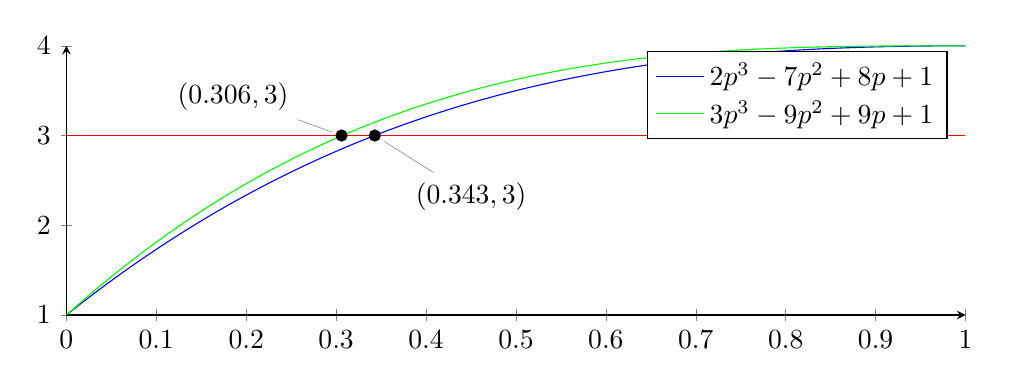
\begin{tikzpicture}
\begin{axis}[
    axis lines = left,
    ytick={1,2,3,4,5},
    xtick={0,0.1,0.2,0.3,0.4,0.5,0.6,0.7,0.8,0.9,1},
    height=5cm,
    width=13cm,
]

\addplot [
    domain=0:1, 
    samples=1000, 
    color=blue,
    ]
    {2*x^3 - 7*x^2 + 8*x + 1};
\addlegendentry{\(2p^{3}-7p^{2}+8p+1\)}

\addplot [
    domain=-0:1, 
    samples=100, 
    color=green,
    ]
    {3*x^3 - 9*x^2 + 9*x + 1};
\addlegendentry{\(3p^3-9p^2+9p+1\)}

\addplot [
    domain=0:1, 
    samples=100, 
    color=red,
    ]
    {3};

\addplot[mark=*] coordinates {(0.306,3)} node[pin=160:{$(0.306,3)$}]{} ;
\addplot[mark=*] coordinates {(0.343,3)} node[pin=310:{$(0.343,3)$}]{} ;

\end{axis}
\end{tikzpicture}
\end{center}
\\
From the graph, we find that in the worse case, when the group size is equal to 3, pooling should be used only when $p<0.306$ such that the expected amount of tests used is lower than the traditional way.
\\
\\
We can compare the two expected functions by considering the difference:
\\
\begin{displaymath}
D(p)=T(p)-t(p)=3p^3-9p^2+9p+1-(2p^{3}-7p^{2}+8p+1)
\end{displaymath}
\\
Solving $D(p):$
\\
\begin{displaymath}
D(p)=-p^2+p
\end{displaymath}
\\
The difference of the two equations is a quadratic equation.
\\
\\
Graphing the equation:
\\
\begin{center}
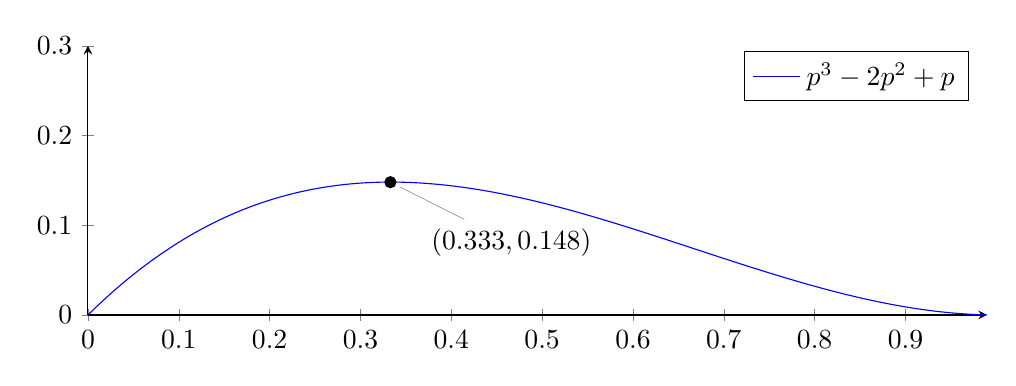
\begin{tikzpicture}
\begin{axis}[
    axis lines = left,
    ytick={0,0.1,0.2,0.3},
    ymin=0.0,ymax=0.3,
    xtick={0,0.1,0.2,0.3,0.4,0.5,0.6,0.7,0.8,0.9,1},
    height=5cm,
    width=13cm,
]

%Here the blue parabola is defined
\addplot [
    domain=0:1, 
    samples=100, 
    color=blue,
    ]
    {x^3 -2*x^2 +x};
\addlegendentry{\(p^3 -2p^2+p\)}

%Two dots are defined
\addplot[mark=*] coordinates {(0.333,0.148)} node[pin=310:{$(0.333,0.148)$}]{} ;

\end{axis}
\end{tikzpicture}
\end{center}
\\
From the graph, we can see that the vertex of the equation is $(0.333,0.148)$, which means that the biggest difference occurs when $p=0.333$ and the expected value of the two models differ by 0.148 tests.